\chapter{Conclusiones y resultados}

\section{Análisis del rendimiento}

Veamos ahora el rendimiento obtenido por esta implementación. Para comparar los resultados obtenidos usaremos el renderer Mitsuba. Se trata de un software open-source desarrollado por investigadores que implementa algunos de los algoritmos y técnicas de renderizado mas pioneras. Mitsuba se ejecuta en la CPU con multithreading y esta altamente optimizado para las arquitecturas de CPU actuales.

\medskip
Para la comparativa se utilizado una CPU Intel Core i7 con 4 núcleos a 2GHz y una GPU Nvidia Geforce GT 740M con 384 núcleos cuda.
\medskip

Con tal de ejecutar algoritmos similares hemos configurado Mitsuba para que ejecute un rendering por pathtracing, que es el mismo algoritmo implementado en este trabajo pero con algunas diferencias, que comentaremos posteriormente.
Ambos programas realizaran un renderizado de una escena idéntica de 66450 triángulos, con una única fuente de luz, sobre un lienzo de 1024x768 pixels.

\clearpage

\begin{figure}[h!]
\centering
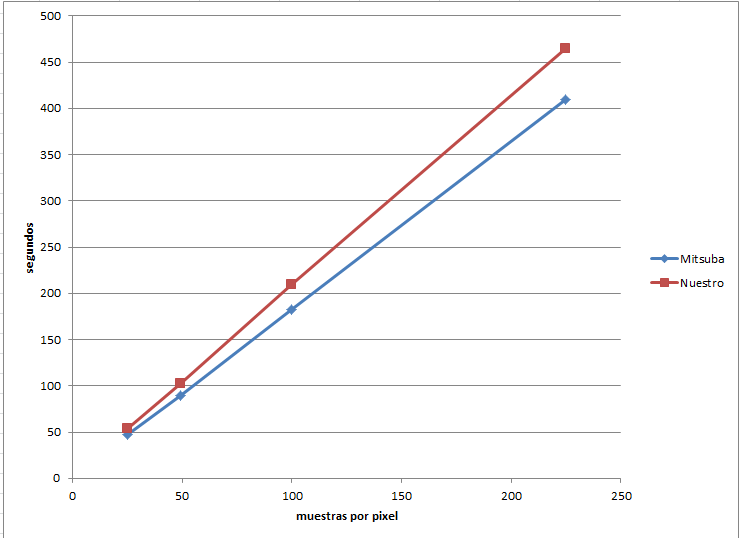
\includegraphics[width=5in]{comparativa_1.png}
\caption{Tiempo de ejecución por número de muestras por pixel con una luz}
\end{figure}

Es evidente que estos resultados no son los esperados. Los tiempos de ejecución de ambos programas son similares pero Mitsuba es ligeramente mas rápido. Hay varios factores que explican este hecho. Una de las diferencias entre la implementación de Mitsuba  y la nuestra es que en su caso el muestreo de luz directa se hace antes de muestrear la BRDF, y en caso de obtener una contribución de luz directa se termina el path. En nuestro caso primero muestreamos la BRDF, lanzamos el rayo indirecto y solo muestreamos la luz directa a la vuelta de la recursión. Esta diferencia produce, en nuestro caso, paths mas largos de media, lo que incrementa el tiempo de ejecución.

\medskip

Además de los factores comentados 


\clearpage

En otra prueba realizada se han utilizado los mismos parámetros de escena pero usando tres fuentes de luz en vez de una. 

\begin{figure}[h]
\centering
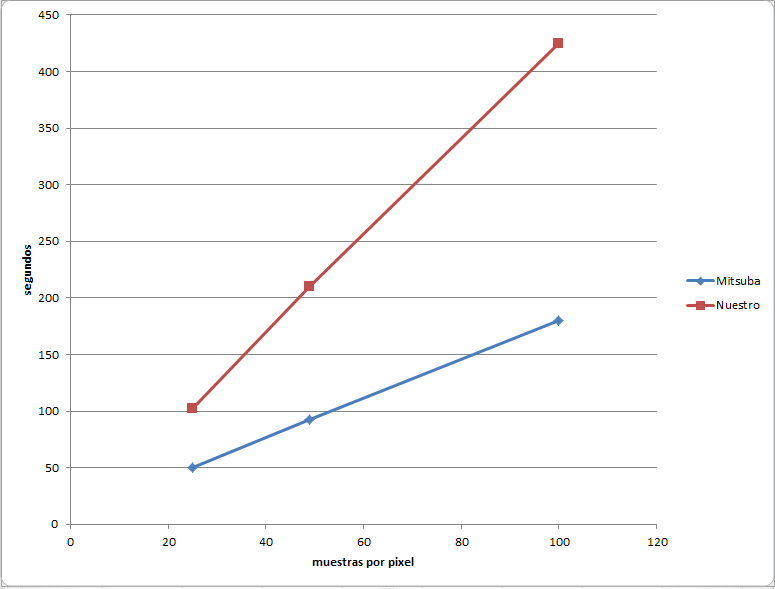
\includegraphics[width=5in]{comparativa_2.png}
\caption{Tiempo de ejecución por número de muestras por pixel con tres luces}
\end{figure}

Esta comparativa es aun mas bizarra que la anterior. Podemos ver que mientras Mitsuba escala bien con el número de luces, nuestro tiempo de ejecución se dispara. Ya que desconocemos el funcionamiento interno de Mitsuba, podemos teorizar que Mitsuba utiliza la versión del algoritmo original propuesta por Kajiya \cite{Kajiya1986}, en la que solo se muestrea una de las luces de la escena aleatoriamente. Por el contrario, nuestra implementación lanza un rayo contra cada luz, por lo que el número de rayos lanzados crece linealmente con el número de luces. 

\medskip
Otros aspectos que pueden haber afectado los resultados son el hardware utilizado en los experimentos y la calidad de la implementación, puesto que Mitsuba ha sido desarrollado y optimizado por investigadores profesionales de la materia y nuestra implementación es una prueba de concepto con muy poca optimización.

\clearpage


\section{Valoración de los resultados obtenidos}


El campo de estudio en el que se sitúa el presente trabajo es muy amplio y ha sido muy estudiado por un gran número de investigadores. A medida que profundizábamos en la materia de estudio iban surgiendo cada vez más detalles, mejoras y variaciones en la teoría que incrementaban el abasto del proyecto y generaban nuevas dudas. Por ello hemos llegado a un punto en el que, por el alcance de un TFG, hemos tenido que empezar a descartar cosas que al autor le hubiese gustado investigar en más profundidad. Aún así, valoramos positivamente los resultados obtenidos, pues se ha alcanzado el objetivo principal de este trabajo que era implementar un algoritmo de renderizado realista. 

\medskip

Basándonos en los resultados de los experimentos no se puede confirmar la hipótesis de que una implementación en la GPU es más rápida que una en la CPU, pero considerando los aspectos comentados y la potencial optimización del código creemos que la hipótesis sigue siendo valida.

\clearpage

\section{Posibles mejoras}

Planteamos tres grupos de posibles mejores bien diferenciados: En primer lugar tenemos las mejoras al algoritmo usado. El algoritmo de path tracing que hemos implementado es una de sus versiones más básicas y tal como hemos comentado en la introducción existen variaciones del mismo que ofrecen mejores resultados en un menor número de muestras. Por ejemplo, una primera mejora sería implementar el transporte de luz bidireccional que ofrecería mejores resultados cuando se trata de iluminar escenas en las que la fuente de luz está muy escondida con respecto a la zona enfocada por la cámara. Otra importante mejora sería explorar e implementar modelos de BRDFs más realistas, pues el que hemos usado es de los más básicos que hay. Además, en este trabajo hemos omitido el importante fenómeno de la refractancia de la luz.

\medskip

Otro grupo de mejoras, más allá de este algoritmo en concreto, sería buscar formas de combinar distintos algoritmos. Aunque en principio el algoritmo utilizado es capaz de simular los fenómenos de la luz más habituales esto no significa que sea el mejor para todos ellos. Existen algoritmos que destacan en simular aspectos específicos del transporte lumínico y un buen motor de renderizado puede aprovechar ese hecho para combinar algoritmos de forma inteligente. Por ejemplo, versiones del algoritmo de radiosity o instant radiosity pueden usarse en una primera fase para computar un mapa de luz difusa de la escena. En una segunda fase se puede utilizar alguna de las variantes de path tracing para calcular la luz especular y la luz refractada, haciendo consultas al mapa de luz difusa cuando sea necesario. Finalmente una ejecución de photon mapping puede usarse para calcular las causticas con un mayor nivel de detalle.
Una buena explicación de este uso combinado de algoritmos se puede encontrar en \cite{Hery2013}.

\medskip

Por último y aunque no era el objetivo de este proyecto, una mejora interesante sería implementar una interfaz de usuario que permitiese configurar la escena de forma fácil y cómoda. Por ejemplo una interfaz con Qt con una vista OpenGL, que permita previsualizar la escena, cargar modelos tridimensionales y colocar las luces y la cámara facilitaría mucho el hecho de configurar escenas y crear nuevos renderizados.

\clearpage

\section{Perspectivas de futuro}

Durante el desarrollo de este proyecto hemos podido comprobar que las ganancias de velocidad al ejecutar el algoritmo de path tracing en la GPU, frente a hacerlo en la CPU, son muy notorias. Con nuestra implementación es posible renderizar escenas de varios millones de polígonos, con cientos de muestras por pixel en unos cuantos minutos. Realizar el mismo tipo de renderizado en una CPU actual podría tardar varios días.

\medskip

Además, considerando que los experimentos se han realizado con una tarjeta gráfica de ordenador portátil y que la implementación es muy optimizable, creemos que en pocos años será habitual disponer de software capaz de renderizar escenas con iluminación global en tiempo real.

\clearpage

\section{Algunos resultados}

\begin{figure}[h]
\centering
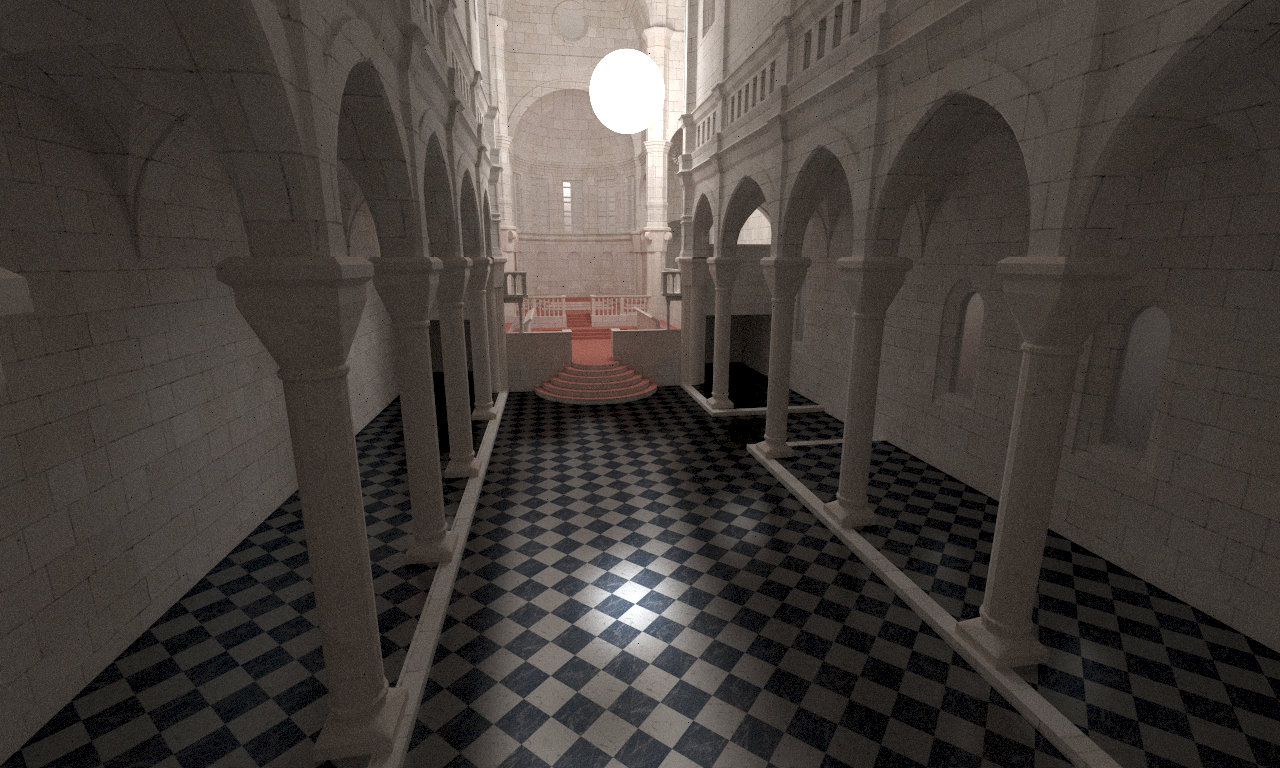
\includegraphics[width=5in]{sibenik_specular.png}
\caption{La textura del suelo es un mapa especular}
\end{figure}

\begin{figure}
\centering
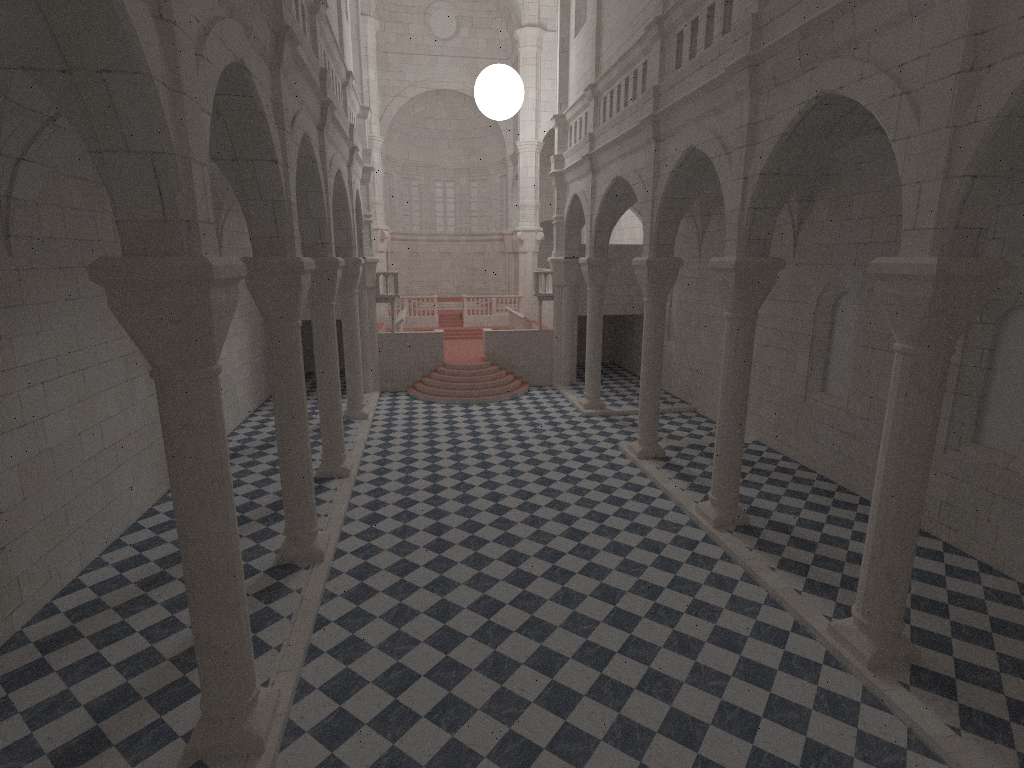
\includegraphics[width=5in]{sibenik_difuse.png}
\caption{La misma escena con un suelo difuso}
\end{figure}

\begin{figure}
\centering
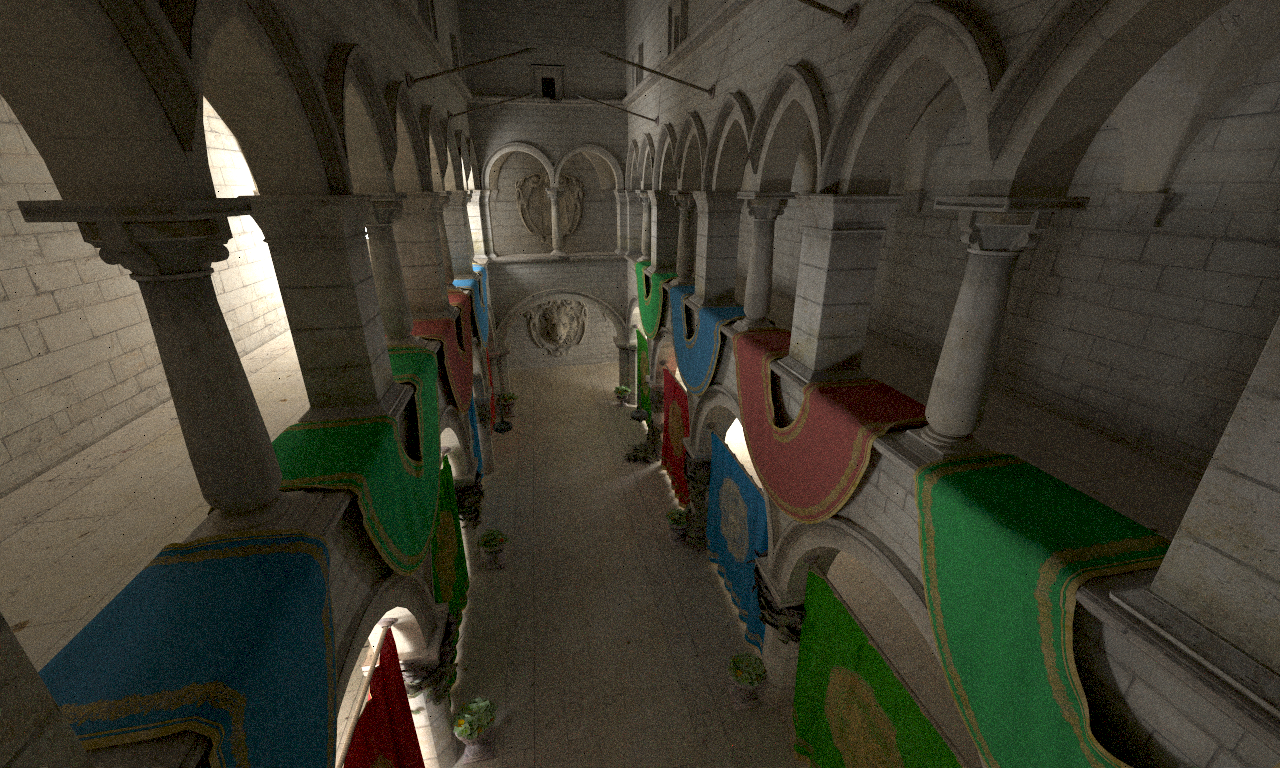
\includegraphics[width=5in]{crytek_sponza1.png}
\caption{Tres fuentes de luz poco visibles iluminan toda la escena}
\end{figure}

\clearpage

\begin{figure}
\centering
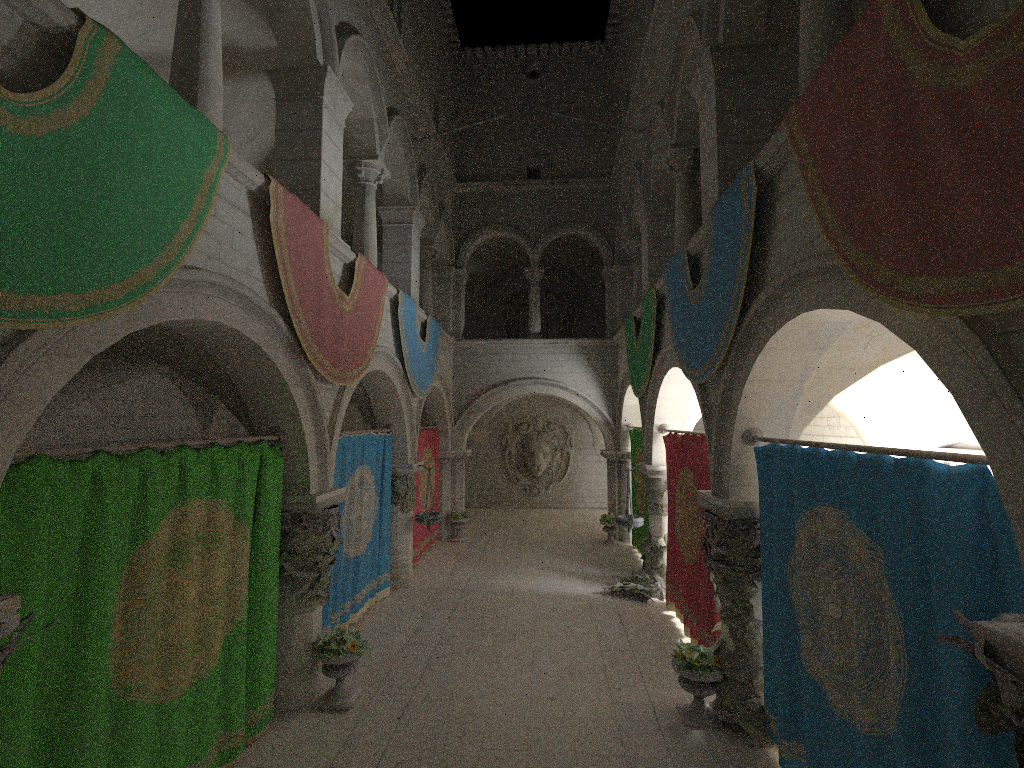
\includegraphics[width=5in]{lion_closer.png}
\caption{La escena anterior desde un ángulo distinto y con una única luz}
\end{figure}

\begin{figure}
\centering
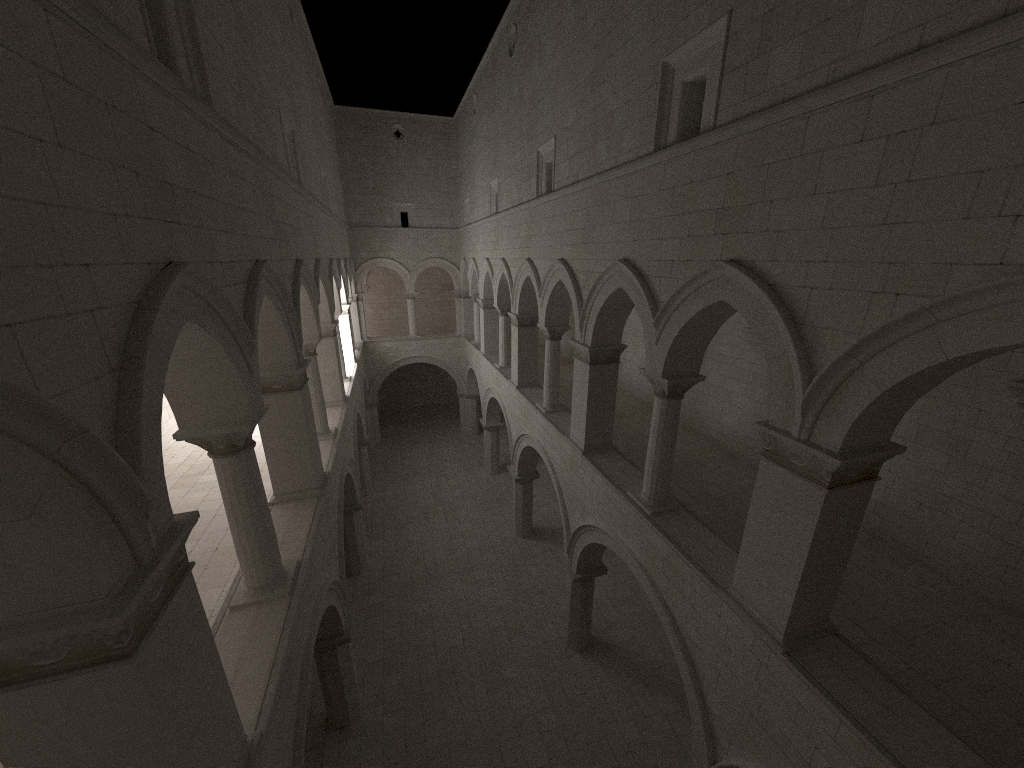
\includegraphics[width=5in]{single_light_sponza.png}
\caption{Iluminación por una única fuente de luz}
\end{figure}

\clearpage

\begin{figure}
\centering
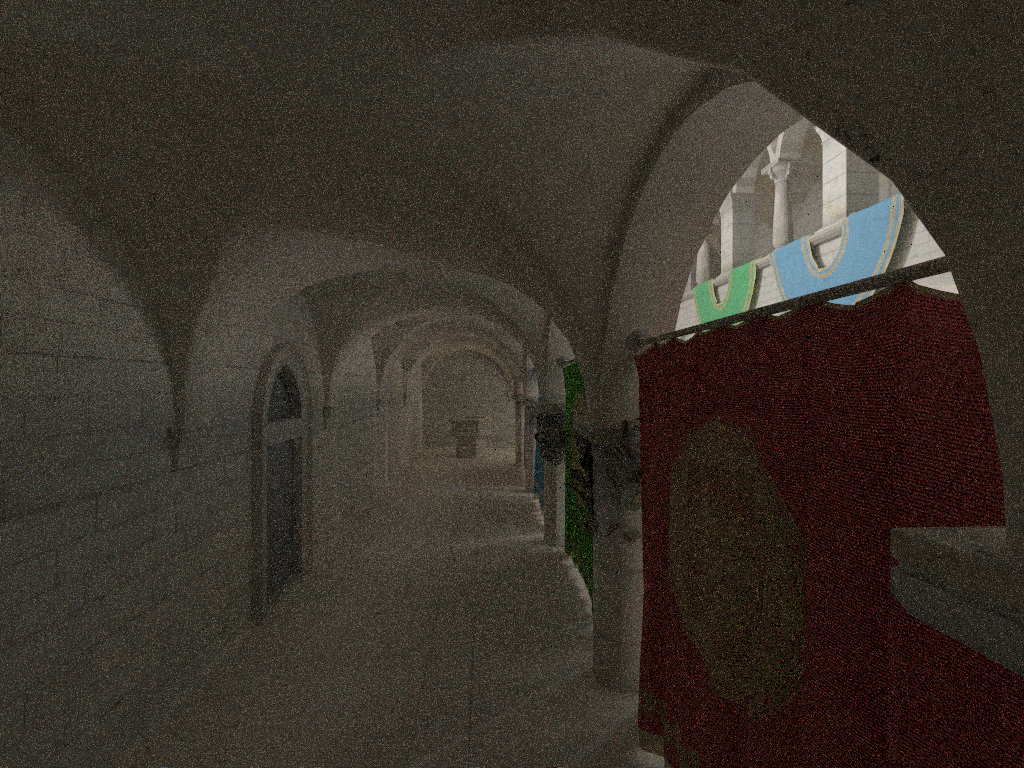
\includegraphics[width=5in]{indirect.png}
\caption{Toda la iluminación del pasillo es luz indirecta debida a rebotes difusos}
\end{figure}

\nocite{Ashikhmin2000}
\nocite{Cook1984}
\nocite{Dutre2003}
\nocite{Torrance1967}
\nocite{Torrance1967}
\nocite{Veach1995}
\nocite{Walter2007}